% Compile standalone, include the resulting PDF in the main report.
\documentclass[border=3pt,tikz]{standalone}
\usepackage{tikz}
\usetikzlibrary{positioning, arrows.meta, calc, fit}

\begin{document}
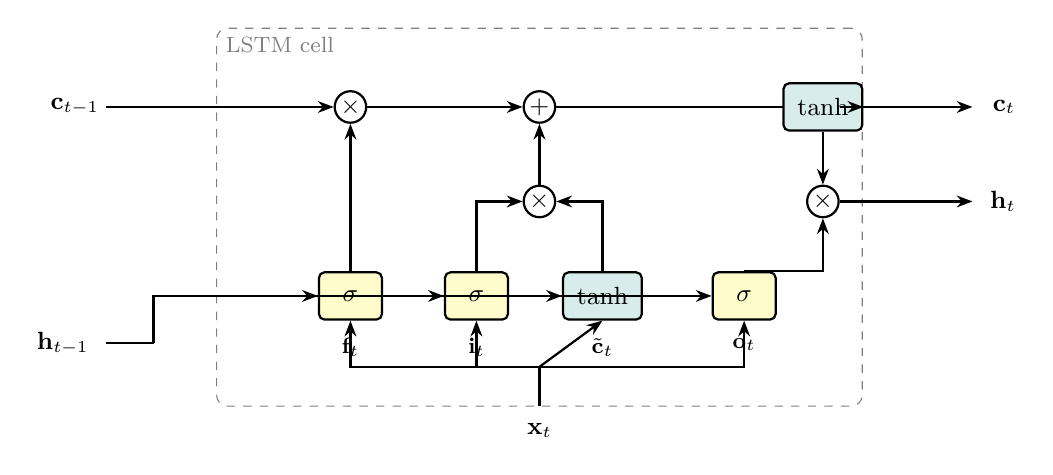
\begin{tikzpicture}[
    >={Stealth[length=2mm]},
    every node/.style = {font=\small},
    gate/.style       = {rectangle, rounded corners=2pt, draw, thick,
                         minimum width=8mm, minimum height=6mm, fill=yellow!20},
    act/.style        = {rectangle, rounded corners=2pt, draw, thick,
                         minimum width=10mm, minimum height=6mm, fill=teal!15},
    op/.style         = {circle, draw, thick, inner sep=0pt, minimum size=4mm},
    line/.style       = {->, thick}
]
% Cell envelope
\node[draw, dashed, gray, rounded corners,
      minimum width=82mm, minimum height=48mm] (cell) at (0,0) {};
\node[anchor=north west, gray] at (cell.north west) {\footnotesize LSTM cell};

% Cell state highway (top)
\coordinate (cL) at (-5.5,1.4);
\coordinate (cR) at ( 5.5,1.4);
\node[left  of=cL, node distance=4mm] {$\mathbf{c}_{t-1}$};
\node[right of=cR, node distance=4mm] {$\mathbf{c}_t$};
\node[op] (mult1) at (-2.4,1.4) {$\times$};
\node[op] (sum)   at ( 0.0,1.4) {$+$};
\draw[line] (cL) -- (mult1);
\draw[line] (mult1) -- (sum);
\draw[line] (sum) -- (cR);

% Gates
\node[gate] (f) at (-2.4,-1.0) {$\sigma$};
\node[gate] (i) at (-0.8,-1.0) {$\sigma$};
\node[act]  (cc) at ( 0.8,-1.0) {$\tanh$};
\node[gate] (o) at ( 2.6,-1.0) {$\sigma$};

\node[below=1mm of f]  {\footnotesize $\mathbf{f}_t$};
\node[below=1mm of i]  {\footnotesize $\mathbf{i}_t$};
\node[below=1mm of cc] {\footnotesize $\tilde{\mathbf{c}}_t$};
\node[below=1mm of o]  {\footnotesize $\mathbf{o}_t$};

% Multiplication of i_t and candidate -> sum
\node[op] (mult2) at (0,0.2) {$\times$};
\draw[line] (i.north) |- (mult2.west);
\draw[line] (cc.north) |- (mult2.east);
\draw[line] (mult2) -- (sum);

% Forget gate -> mult1
\draw[line] (f.north) -- (mult1.south);

% Output path: cell state -> tanh -> mult3 -> h_t
\node[act] (tanhOut) at (3.6,1.4) {$\tanh$};
\node[op]  (mult3)   at (3.6,0.2) {$\times$};
\draw[line] (cR -| tanhOut.east) ++(-0.3,0) coordinate (tap) -- (tanhOut);
\draw[line] (tanhOut) -- (mult3);
\draw[line] (o.north) -| (mult3.south);

% h_t and c_t outputs
\coordinate (htOut) at (5.5,0.2);
\draw[line] (mult3) -- (htOut);
\node[right=1mm of htOut] {$\mathbf{h}_t$};

% Inputs h_{t-1} and x_t
\coordinate (hin) at (-5.5,-1.6);
\node[left=1mm of hin] {$\mathbf{h}_{t-1}$};
\coordinate (xin) at (0, -2.4);
\node[below=1mm of xin] {$\mathbf{x}_t$};

% h_{t-1} fan-out
\draw[thick] (hin) -- ++(0.6,0) coordinate (hbus);
\draw[line] (hbus) |- (f.west);
\draw[line] (hbus) |- (i.west);
\draw[line] (hbus) |- (cc.west);
\draw[line] (hbus) |- (o.west);

% x_t fan-out
\draw[thick] (xin) -- (0,-1.9) coordinate (xbus);
\draw[line] (xbus) -| (f.south);
\draw[line] (xbus) -| (i.south);
\draw[line] (xbus) -- (cc.south);
\draw[line] (xbus) -| (o.south);

\end{tikzpicture}
\end{document}